% Options for packages loaded elsewhere
\PassOptionsToPackage{unicode}{hyperref}
\PassOptionsToPackage{hyphens}{url}
%
\documentclass[
]{book}
\usepackage{amsmath,amssymb}
\usepackage{lmodern}
\usepackage{ifxetex,ifluatex}
\ifnum 0\ifxetex 1\fi\ifluatex 1\fi=0 % if pdftex
  \usepackage[T1]{fontenc}
  \usepackage[utf8]{inputenc}
  \usepackage{textcomp} % provide euro and other symbols
\else % if luatex or xetex
  \usepackage{unicode-math}
  \defaultfontfeatures{Scale=MatchLowercase}
  \defaultfontfeatures[\rmfamily]{Ligatures=TeX,Scale=1}
\fi
% Use upquote if available, for straight quotes in verbatim environments
\IfFileExists{upquote.sty}{\usepackage{upquote}}{}
\IfFileExists{microtype.sty}{% use microtype if available
  \usepackage[]{microtype}
  \UseMicrotypeSet[protrusion]{basicmath} % disable protrusion for tt fonts
}{}
\makeatletter
\@ifundefined{KOMAClassName}{% if non-KOMA class
  \IfFileExists{parskip.sty}{%
    \usepackage{parskip}
  }{% else
    \setlength{\parindent}{0pt}
    \setlength{\parskip}{6pt plus 2pt minus 1pt}}
}{% if KOMA class
  \KOMAoptions{parskip=half}}
\makeatother
\usepackage{xcolor}
\IfFileExists{xurl.sty}{\usepackage{xurl}}{} % add URL line breaks if available
\IfFileExists{bookmark.sty}{\usepackage{bookmark}}{\usepackage{hyperref}}
\hypersetup{
  pdftitle={Visualisering af biologiske datasæt},
  pdfauthor={Sarah Rennie},
  hidelinks,
  pdfcreator={LaTeX via pandoc}}
\urlstyle{same} % disable monospaced font for URLs
\usepackage{color}
\usepackage{fancyvrb}
\newcommand{\VerbBar}{|}
\newcommand{\VERB}{\Verb[commandchars=\\\{\}]}
\DefineVerbatimEnvironment{Highlighting}{Verbatim}{commandchars=\\\{\}}
% Add ',fontsize=\small' for more characters per line
\usepackage{framed}
\definecolor{shadecolor}{RGB}{248,248,248}
\newenvironment{Shaded}{\begin{snugshade}}{\end{snugshade}}
\newcommand{\AlertTok}[1]{\textcolor[rgb]{0.94,0.16,0.16}{#1}}
\newcommand{\AnnotationTok}[1]{\textcolor[rgb]{0.56,0.35,0.01}{\textbf{\textit{#1}}}}
\newcommand{\AttributeTok}[1]{\textcolor[rgb]{0.77,0.63,0.00}{#1}}
\newcommand{\BaseNTok}[1]{\textcolor[rgb]{0.00,0.00,0.81}{#1}}
\newcommand{\BuiltInTok}[1]{#1}
\newcommand{\CharTok}[1]{\textcolor[rgb]{0.31,0.60,0.02}{#1}}
\newcommand{\CommentTok}[1]{\textcolor[rgb]{0.56,0.35,0.01}{\textit{#1}}}
\newcommand{\CommentVarTok}[1]{\textcolor[rgb]{0.56,0.35,0.01}{\textbf{\textit{#1}}}}
\newcommand{\ConstantTok}[1]{\textcolor[rgb]{0.00,0.00,0.00}{#1}}
\newcommand{\ControlFlowTok}[1]{\textcolor[rgb]{0.13,0.29,0.53}{\textbf{#1}}}
\newcommand{\DataTypeTok}[1]{\textcolor[rgb]{0.13,0.29,0.53}{#1}}
\newcommand{\DecValTok}[1]{\textcolor[rgb]{0.00,0.00,0.81}{#1}}
\newcommand{\DocumentationTok}[1]{\textcolor[rgb]{0.56,0.35,0.01}{\textbf{\textit{#1}}}}
\newcommand{\ErrorTok}[1]{\textcolor[rgb]{0.64,0.00,0.00}{\textbf{#1}}}
\newcommand{\ExtensionTok}[1]{#1}
\newcommand{\FloatTok}[1]{\textcolor[rgb]{0.00,0.00,0.81}{#1}}
\newcommand{\FunctionTok}[1]{\textcolor[rgb]{0.00,0.00,0.00}{#1}}
\newcommand{\ImportTok}[1]{#1}
\newcommand{\InformationTok}[1]{\textcolor[rgb]{0.56,0.35,0.01}{\textbf{\textit{#1}}}}
\newcommand{\KeywordTok}[1]{\textcolor[rgb]{0.13,0.29,0.53}{\textbf{#1}}}
\newcommand{\NormalTok}[1]{#1}
\newcommand{\OperatorTok}[1]{\textcolor[rgb]{0.81,0.36,0.00}{\textbf{#1}}}
\newcommand{\OtherTok}[1]{\textcolor[rgb]{0.56,0.35,0.01}{#1}}
\newcommand{\PreprocessorTok}[1]{\textcolor[rgb]{0.56,0.35,0.01}{\textit{#1}}}
\newcommand{\RegionMarkerTok}[1]{#1}
\newcommand{\SpecialCharTok}[1]{\textcolor[rgb]{0.00,0.00,0.00}{#1}}
\newcommand{\SpecialStringTok}[1]{\textcolor[rgb]{0.31,0.60,0.02}{#1}}
\newcommand{\StringTok}[1]{\textcolor[rgb]{0.31,0.60,0.02}{#1}}
\newcommand{\VariableTok}[1]{\textcolor[rgb]{0.00,0.00,0.00}{#1}}
\newcommand{\VerbatimStringTok}[1]{\textcolor[rgb]{0.31,0.60,0.02}{#1}}
\newcommand{\WarningTok}[1]{\textcolor[rgb]{0.56,0.35,0.01}{\textbf{\textit{#1}}}}
\usepackage{longtable,booktabs,array}
\usepackage{calc} % for calculating minipage widths
% Correct order of tables after \paragraph or \subparagraph
\usepackage{etoolbox}
\makeatletter
\patchcmd\longtable{\par}{\if@noskipsec\mbox{}\fi\par}{}{}
\makeatother
% Allow footnotes in longtable head/foot
\IfFileExists{footnotehyper.sty}{\usepackage{footnotehyper}}{\usepackage{footnote}}
\makesavenoteenv{longtable}
\usepackage{graphicx}
\makeatletter
\def\maxwidth{\ifdim\Gin@nat@width>\linewidth\linewidth\else\Gin@nat@width\fi}
\def\maxheight{\ifdim\Gin@nat@height>\textheight\textheight\else\Gin@nat@height\fi}
\makeatother
% Scale images if necessary, so that they will not overflow the page
% margins by default, and it is still possible to overwrite the defaults
% using explicit options in \includegraphics[width, height, ...]{}
\setkeys{Gin}{width=\maxwidth,height=\maxheight,keepaspectratio}
% Set default figure placement to htbp
\makeatletter
\def\fps@figure{htbp}
\makeatother
\setlength{\emergencystretch}{3em} % prevent overfull lines
\providecommand{\tightlist}{%
  \setlength{\itemsep}{0pt}\setlength{\parskip}{0pt}}
\setcounter{secnumdepth}{5}
\usepackage{booktabs}
\ifluatex
  \usepackage{selnolig}  % disable illegal ligatures
\fi
\usepackage[]{natbib}
\bibliographystyle{apalike}

\title{Visualisering af biologiske datasæt}
\author{Sarah Rennie}
\date{2022-02-21}

\begin{document}
\maketitle

{
\setcounter{tocdepth}{1}
\tableofcontents
}
\hypertarget{basics}{%
\chapter{Grundlæggende R}\label{basics}}

\hypertarget{inledning-til-kapitel}{%
\section{Inledning til kapitel}\label{inledning-til-kapitel}}

Jeg har prøvet at opsummere nogle grundlæggende ting, som I skal vide før vi går videre i kurset. Derefter er der nogle problemstillinger som jeg anbefaler at I arbejder igennem, for at tjekke jeres forståelse af koncepterne og udfylder eventuelle huller i jeres viden.

Det er helt fint, hvis I ikke har set de hele før. Skrive til mig gerne, hvis I har nogle spørgsmål, som vi kan diskutere i vores næste lektion.

\hypertarget{rstudio}{%
\section{Rstudio}\label{rstudio}}

Det allerførste man skulle gør, hvis man ikke har brugt RStudio før, er at downloade den gratis på nettet:

\url{https://www.rstudio.com/products/rstudio/download/\#download}

Vi kommer fremadrettet til at være meget afhængig af nogle af dets funktionalitet til at lave blandt andet R Markdown dokumenter. R Markdown bliver præsenteret i vores næste lektion.

\hypertarget{de-forskellige-vinduer-i-rstudio}{%
\subsection{De forskellige vinduer i RStudio}\label{de-forskellige-vinduer-i-rstudio}}

Hvis man ikke har et kendskab til RStudio, kan man tjekke det her for at lære de forskellige vinduer at kende:

\url{https://bookdown.org/ndphillips/YaRrr/the-four-rstudio-windows.html}

\begin{itemize}
\tightlist
\item
  Man skrive kode i Source (øverst til venstre)
\item
  Man kører kode ved at tryk CMD+ENTER (eller WIN-KEY+ENTER)
\item
  Kode køres ind i Console (som plejer at være nederst til venstre, selvom det er øverst til højere i billedet).
\item
  Environment - her kan man se, alle objekter i workspace-en.
\end{itemize}

\hypertarget{suxe6tte-working-directory}{%
\section{Sætte working directory}\label{suxe6tte-working-directory}}

Når man arbejde på et projekt, er det nyttigt at vide, den \emph{working directory} som R arbejder fra - det er det sted, hvor R forsøger at åbne eller gemme filer, medmindre man angiver et andet path.

\begin{Shaded}
\begin{Highlighting}[]
\FunctionTok{getwd}\NormalTok{() }\CommentTok{\#se nuværende working directory}
\FunctionTok{list.dirs}\NormalTok{(}\AttributeTok{path =} \StringTok{"."}\NormalTok{, }\AttributeTok{recursive =} \ConstantTok{FALSE}\NormalTok{) }\CommentTok{\#se mappe indenfor working directory}
\FunctionTok{setwd}\NormalTok{(}\StringTok{"\textasciitilde{}/Documents/"}\NormalTok{) }\CommentTok{\#sætte en ny working directory (C:/Users/myname/Documents hvis man bruger Windows)}
\end{Highlighting}
\end{Shaded}

\hypertarget{r-pakker}{%
\section{R pakker}\label{r-pakker}}

R pakker er simpelthen en samling af funktioner (eller datasæt), som udvider hvad er tilgængelige i base-R (den R man få, uden at indlæse nogle som helst pakke). I R er der mange tusind R pakke (faktisk op mod 100,000), som plejer at være tilgængelige på \textbf{CRAN} (\url{https://cran.r-project.org/}). Indenfor biologiske fag er der også mange flere på \textbf{Bioconductor} (\url{https://www.bioconductor.org/}), og nogle gange er R-pakke også installeret direkte fra \textbf{Github}.

I dette kursus arbejder vi rigtig meget med en pakke der hedder \textbf{tidyverse}. Før man indlæse det, skal man først sikre sig, at pakken er installeret på systemet:

\begin{Shaded}
\begin{Highlighting}[]
\FunctionTok{install.packages}\NormalTok{(}\StringTok{"tidyverse"}\NormalTok{)}
\end{Highlighting}
\end{Shaded}

Alle pakker på \textbf{CRAN} er installeret på samme måde. Når man bruger en R pakke, skal man først indlæse den ved at bruge \texttt{library()}:

\begin{Shaded}
\begin{Highlighting}[]
\FunctionTok{library}\NormalTok{(tidyverse)}
\end{Highlighting}
\end{Shaded}

\begin{verbatim}
## -- Attaching packages --------------------------------------- tidyverse 1.3.1 --
\end{verbatim}

\begin{verbatim}
## v ggplot2 3.3.5     v purrr   0.3.4
## v tibble  3.1.2     v dplyr   1.0.7
## v tidyr   1.1.3     v stringr 1.4.0
## v readr   1.4.0     v forcats 0.5.1
\end{verbatim}

\begin{verbatim}
## -- Conflicts ------------------------------------------ tidyverse_conflicts() --
## x dplyr::filter() masks stats::filter()
## x dplyr::lag()    masks stats::lag()
\end{verbatim}

I dette tilfælde kan man se, at \textbf{tidyverse} er faktisk en samling af otte andre pakke, som blev indlæste. Vi kommer til at arbejde med disse pakker fra kapitel tre (vi starter med \textbf{ggplot2} og så nogle af de andre pakke fra \textbf{tidyverse} fra kapitel fire)

\hypertarget{hvor-kommer-data-fra}{%
\section{Hvor kommer data fra?}\label{hvor-kommer-data-fra}}

De data, vi arbejde med i kurset stammer fra forskellige steder.

\hypertarget{indbygget-datasuxe6t}{%
\subsection{Indbygget datasæt}\label{indbygget-datasuxe6t}}

I R er der mange indbygget datasæt som er meget brugbare for at vise eller lege med koncepter, som især gøre dem populære for undervisningsmateriale. Indbygget datasæt kan være tilgænglige indenfor mange pakke, men \texttt{library(datasets)} er den mest brugt (der er også mange indenfor \texttt{library(ggplot2)}. For eksempel, for at indlæse datasættet, der hedder `iris', kan man bruge \texttt{data()}:

\begin{Shaded}
\begin{Highlighting}[]
\FunctionTok{library}\NormalTok{(datasets)}
\FunctionTok{data}\NormalTok{(iris)}
\end{Highlighting}
\end{Shaded}

Så er en \emph{dataramme} tilgængelige som en \emph{objekt} i \emph{workspacen} - se ``Environment'' fane på højere side i RStudio, eller indtaste \texttt{ls()}, så bør du kunne se en objekt med navn `iris'. Man kan kun arbejde med objekter som er en del af workspacen.

\hypertarget{importering-af-data-fra-.txt-fil}{%
\subsection{Importering af data fra .txt fil}\label{importering-af-data-fra-.txt-fil}}

Det er meget hyppigt, at man har sin data i formen af en .txt fil eller .xlsx fil på sin computer. Den nemmeste måde at få åbnet en .txt fil er ved at bruge \texttt{read.table()}, som i nedenstående:

\begin{Shaded}
\begin{Highlighting}[]
\NormalTok{data }\OtherTok{\textless{}{-}} \FunctionTok{read.table}\NormalTok{(}\StringTok{"mydata.txt"}\NormalTok{) }\CommentTok{\#indlæse data filen mydata.txt som er i working directory}
\FunctionTok{head}\NormalTok{(data)}
\end{Highlighting}
\end{Shaded}

Huske at hvis data har kolonner navne, så skal man bruge \texttt{header=T} for at undgå, at den første række i data bliver disse navne i stedet for virkelige observationer.

\begin{Shaded}
\begin{Highlighting}[]
\NormalTok{data }\OtherTok{\textless{}{-}} \FunctionTok{read.table}\NormalTok{(}\StringTok{"mydata.txt"}\NormalTok{,}\AttributeTok{header=}\NormalTok{T) }\CommentTok{\#indlæse data filen mydata.txt som er i working directory}
\FunctionTok{head}\NormalTok{(data)}
\end{Highlighting}
\end{Shaded}

\hypertarget{importering-af-data-fra-excel}{%
\subsection{Importering af data fra Excel}\label{importering-af-data-fra-excel}}

Der findes også en hjælpsom pakke, der kan indlæse Excel-ark direkte ind i R:

\begin{Shaded}
\begin{Highlighting}[]
\FunctionTok{library}\NormalTok{(readxl)}
\NormalTok{data }\OtherTok{\textless{}{-}} \FunctionTok{read\_excel}\NormalTok{(}\StringTok{"data.xlsx"}\NormalTok{)}
\NormalTok{data}
\end{Highlighting}
\end{Shaded}

\hypertarget{dataramme-koncepter}{%
\section{Dataramme koncepter}\label{dataramme-koncepter}}

\url{http://www.r-tutor.com/r-introduction/data-frame}

Mange af de ting, som vi laver i R tager udgangspunkten i datarammer.

\begin{Shaded}
\begin{Highlighting}[]
\NormalTok{mydf }\OtherTok{\textless{}{-}} \FunctionTok{data.frame}\NormalTok{(}\StringTok{"person ID"}\OtherTok{=}\DecValTok{1}\SpecialCharTok{:}\DecValTok{5}\NormalTok{, }\StringTok{"height"}\OtherTok{=}\FunctionTok{c}\NormalTok{(}\DecValTok{140}\NormalTok{,}\DecValTok{187}\NormalTok{,}\DecValTok{154}\NormalTok{,}\DecValTok{132}\NormalTok{,}\DecValTok{165}\NormalTok{), }\StringTok{"age"}\OtherTok{=}\FunctionTok{c}\NormalTok{(}\DecValTok{34}\NormalTok{,}\DecValTok{31}\NormalTok{,}\DecValTok{25}\NormalTok{,}\DecValTok{43}\NormalTok{,}\DecValTok{29}\NormalTok{))}
\NormalTok{mydf}
\end{Highlighting}
\end{Shaded}

\begin{verbatim}
##   person.ID height age
## 1         1    140  34
## 2         2    187  31
## 3         3    154  25
## 4         4    132  43
## 5         5    165  29
\end{verbatim}

Huske, at vores \texttt{data.frame}, ligesom et matrix (i R: \texttt{matrix()}) har to dimensioner - række og kolonner Forskellen mellem en matrix og en dataramme er, at datarammer kan indeholde mange forskellige data typer (herunder numeriske, faktorer, karakterer osv.), men matrix indeholder kun numeriske data. For eksempel

\begin{Shaded}
\begin{Highlighting}[]
\NormalTok{mydf}\SpecialCharTok{$}\NormalTok{colour }\OtherTok{\textless{}{-}} \FunctionTok{c}\NormalTok{(}\StringTok{"red"}\NormalTok{,}\StringTok{"blue"}\NormalTok{,}\StringTok{"green"}\NormalTok{,}\StringTok{"orange"}\NormalTok{,}\StringTok{"purple"}\NormalTok{)}
\NormalTok{mydf}
\end{Highlighting}
\end{Shaded}

\begin{verbatim}
##   person.ID height age colour
## 1         1    140  34    red
## 2         2    187  31   blue
## 3         3    154  25  green
## 4         4    132  43 orange
## 5         5    165  29 purple
\end{verbatim}

er en dataramme med forskellige data type men følgende er en matrix

\begin{Shaded}
\begin{Highlighting}[]
\FunctionTok{matrix}\NormalTok{(}\FunctionTok{c}\NormalTok{(}\DecValTok{1}\NormalTok{, }\DecValTok{2}\NormalTok{, }\DecValTok{3}\NormalTok{, }\DecValTok{4}\NormalTok{, }\DecValTok{5}\NormalTok{, }\DecValTok{6}\NormalTok{), }
    \AttributeTok{nrow=}\DecValTok{3}\NormalTok{,}
    \AttributeTok{ncol=}\DecValTok{2}\NormalTok{)}
\end{Highlighting}
\end{Shaded}

\begin{verbatim}
##      [,1] [,2]
## [1,]    1    4
## [2,]    2    5
## [3,]    3    6
\end{verbatim}

med kun numeriske data, som kan bruges til matematik operationer (matrix multiplikation osv.). I dette kursus beskæftiger os primært med datarammer.

Man kan kigge på en subset af rækkerne i de data ved at

\begin{Shaded}
\begin{Highlighting}[]
\NormalTok{mydf[mydf}\SpecialCharTok{$}\NormalTok{height}\SpecialCharTok{\textgreater{}=}\DecValTok{165}\NormalTok{,] }\CommentTok{\#alle rækker i datarammen med height = 165 eller over}
\end{Highlighting}
\end{Shaded}

\begin{verbatim}
##   person.ID height age colour
## 2         2    187  31   blue
## 5         5    165  29 purple
\end{verbatim}

Her i kurset arbejder vi på noget der hedder et `tibble'. Det får vi at vide mere om senere.

\begin{Shaded}
\begin{Highlighting}[]
\NormalTok{mydf\_tibble }\OtherTok{\textless{}{-}} \FunctionTok{tibble}\NormalTok{(mydf)}
\NormalTok{mydf\_tibble}
\end{Highlighting}
\end{Shaded}

\begin{verbatim}
## # A tibble: 5 x 4
##   person.ID height   age colour
##       <int>  <dbl> <dbl> <chr> 
## 1         1    140    34 red   
## 2         2    187    31 blue  
## 3         3    154    25 green 
## 4         4    132    43 orange
## 5         5    165    29 purple
\end{verbatim}

\hypertarget{descriptive-statistics}{%
\section{Descriptive statistics}\label{descriptive-statistics}}

\hypertarget{simulere-data-fra-distributions}{%
\subsection{Simulere data fra distributions}\label{simulere-data-fra-distributions}}

Se for eksempel:

\url{http://www.r-tutor.com/elementary-statistics/probability-distributions/normal-distribution}

Man kan nemt lave sin egne `fake' data ved at simulere det fra nogle distributioner. Det vil typiske være den normale distribution, idet den normale distribution opstå mest hyppigt i den virkelige verden (huske den klassiske klokke-form). I R kan man bruge funktionen \texttt{rnorm} til at simulere data - først angiver man, hvor mange observationer man vil have, og så den mean og standard deviation, som er de to parametre som er nødvendige til at beskrive en normal distribution.

\begin{Shaded}
\begin{Highlighting}[]
\NormalTok{x }\OtherTok{\textless{}{-}} \FunctionTok{rnorm}\NormalTok{(}\DecValTok{25}\NormalTok{,}\AttributeTok{mean=}\DecValTok{0}\NormalTok{,}\AttributeTok{sd=}\DecValTok{1}\NormalTok{) }\CommentTok{\#standard normal distribution}
\NormalTok{x }\CommentTok{\#så har vi 25 værdier fra en normal distribution med mean=0 og standard deviation=1.}
\end{Highlighting}
\end{Shaded}

\begin{verbatim}
##  [1]  0.66705324 -1.28047497  0.54987317  0.51085239 -1.14952601  0.07188865
##  [7]  0.61563390  0.31238346 -0.29262857 -0.27051935  0.22063605  1.48022276
## [13]  0.14809493 -0.05053194  0.05219344  1.48701663 -1.58118898 -0.77298599
## [19]  0.11534840 -0.58103809  1.16270069  1.31932455 -0.06933115 -0.45496956
## [25]  0.67189632
\end{verbatim}

Her har vi kun 25 værdier, men hvis dataen er store, måske vil vi hellere kun kigge på de første (eller sidste) værdier:

\begin{Shaded}
\begin{Highlighting}[]
\FunctionTok{head}\NormalTok{(x) }\CommentTok{\#første 6}
\end{Highlighting}
\end{Shaded}

\begin{verbatim}
## [1]  0.66705324 -1.28047497  0.54987317  0.51085239 -1.14952601  0.07188865
\end{verbatim}

\begin{Shaded}
\begin{Highlighting}[]
\FunctionTok{tail}\NormalTok{(x) }\CommentTok{\#sidste 6}
\end{Highlighting}
\end{Shaded}

\begin{verbatim}
## [1] -0.58103809  1.16270069  1.31932455 -0.06933115 -0.45496956  0.67189632
\end{verbatim}

\begin{Shaded}
\begin{Highlighting}[]
\NormalTok{x[}\DecValTok{1}\NormalTok{] }\CommentTok{\#første værdi}
\end{Highlighting}
\end{Shaded}

\begin{verbatim}
## [1] 0.6670532
\end{verbatim}

\begin{Shaded}
\begin{Highlighting}[]
\NormalTok{x[}\FunctionTok{length}\NormalTok{(x)] }\CommentTok{\#sidste data point}
\end{Highlighting}
\end{Shaded}

\begin{verbatim}
## [1] 0.6718963
\end{verbatim}

Bemærk, at til forskellen af Python og mange andre programmering sprog, R bruger 1-baserende indicer - det betyder, at den første værdi er \texttt{x{[}1{]}} og \textbf{ikke} \texttt{x{[}0{]}} som i Python.

\hypertarget{measures-of-central-tendency}{%
\subsection{Measures of central tendency}\label{measures-of-central-tendency}}

\begin{longtable}[]{@{}ll@{}}
\toprule
function & Description \\
\midrule
\endhead
\texttt{mean()} & mean \(\bar{x}_{i} = \frac{1}{n}\sum_{i=1}^{n} x_{i}\) \\
\texttt{median()} & median value \\
\texttt{max()} & maximum value \\
\texttt{min()} & minimum value \\
\texttt{var()} & variance \(s^2 = \frac{1}{n-1}\sum_{i=1}^{n} (x_{i} - \bar{x}_{i})^2\) \\
\texttt{sd()} & standard deviation \(s\) \\
\bottomrule
\end{longtable}

Lad os afprøve dem på vores simulerede data:

\begin{Shaded}
\begin{Highlighting}[]
\NormalTok{my\_mean }\OtherTok{\textless{}{-}} \FunctionTok{mean}\NormalTok{(x)}
\NormalTok{my\_median }\OtherTok{\textless{}{-}} \FunctionTok{median}\NormalTok{(x)}
\NormalTok{my\_max }\OtherTok{\textless{}{-}} \FunctionTok{max}\NormalTok{(x)}
\NormalTok{my\_min }\OtherTok{\textless{}{-}} \FunctionTok{min}\NormalTok{(x)}
\NormalTok{my\_var }\OtherTok{\textless{}{-}} \FunctionTok{var}\NormalTok{(x)}
\NormalTok{my\_sd }\OtherTok{\textless{}{-}} \FunctionTok{sd}\NormalTok{(x)}
\FunctionTok{c}\NormalTok{(my\_mean,my\_median,my\_max,my\_min,my\_var,my\_sd)}
\end{Highlighting}
\end{Shaded}

\begin{verbatim}
## [1]  0.1152770  0.1153484  1.4870166 -1.5811890  0.6650062  0.8154791
\end{verbatim}

Man kan også lave et summary af dataen, som bestå af mange af de statistiker navnt ovenpå:

\begin{Shaded}
\begin{Highlighting}[]
\FunctionTok{summary}\NormalTok{(x)}
\end{Highlighting}
\end{Shaded}

\begin{verbatim}
##    Min. 1st Qu.  Median    Mean 3rd Qu.    Max. 
## -1.5812 -0.2926  0.1153  0.1153  0.6156  1.4870
\end{verbatim}

\hypertarget{tapply}{%
\subsection{\texorpdfstring{\texttt{tapply()}}{tapply()}}\label{tapply}}

En meget brugbart funktion, som er værd at vide, er \texttt{tapply()}.

\begin{Shaded}
\begin{Highlighting}[]
\FunctionTok{data}\NormalTok{(iris)}
\FunctionTok{tapply}\NormalTok{(iris}\SpecialCharTok{$}\NormalTok{Sepal.Length,iris}\SpecialCharTok{$}\NormalTok{Species,mean) }\CommentTok{\# ovenstående i kun en linje}
\end{Highlighting}
\end{Shaded}

\begin{verbatim}
##     setosa versicolor  virginica 
##      5.006      5.936      6.588
\end{verbatim}

Her tager vi en variabel der hedder \texttt{Sepal.Length}, opdele den i henhold til \texttt{Species}, og beregner \texttt{mean} for enhver af de tre \texttt{Species} (setosa, versicolor og virginica). Man kan opnå det samme resultat ved at beregne \texttt{mean} for de tre \texttt{Species} hver for sig:

\begin{Shaded}
\begin{Highlighting}[]
\CommentTok{\# gennemsnit Sepal Length for Species setosa}
\NormalTok{mean\_setosa }\OtherTok{\textless{}{-}} \FunctionTok{mean}\NormalTok{(iris}\SpecialCharTok{$}\NormalTok{Sepal.Length[iris}\SpecialCharTok{$}\NormalTok{Species}\SpecialCharTok{==}\StringTok{"setosa"}\NormalTok{])}

\CommentTok{\# gennemsnit Sepal Length for Species versicolor}
\NormalTok{mean\_versi }\OtherTok{\textless{}{-}} \FunctionTok{mean}\NormalTok{(iris}\SpecialCharTok{$}\NormalTok{Sepal.Length[iris}\SpecialCharTok{$}\NormalTok{Species}\SpecialCharTok{==}\StringTok{"versicolor"}\NormalTok{]) }

\CommentTok{\# gennemsnit Sepal Length for Species virginica}
\NormalTok{mean\_virgin }\OtherTok{\textless{}{-}} \FunctionTok{mean}\NormalTok{(iris}\SpecialCharTok{$}\NormalTok{Sepal.Length[iris}\SpecialCharTok{$}\NormalTok{Species}\SpecialCharTok{==}\StringTok{"virginica"}\NormalTok{])}

\FunctionTok{c}\NormalTok{(mean\_setosa,mean\_versi,mean\_virgin)}
\end{Highlighting}
\end{Shaded}

\begin{verbatim}
## [1] 5.006 5.936 6.588
\end{verbatim}

Hvis der er mange grupper, så er der en stor fordele ved at brug \texttt{tapply} her. Det er også værd at ved koncepten, fordi vi kommer til lære en lignende koncept i \textbf{tidyverse} (med \texttt{group\_by} og \texttt{summarise}).

\hypertarget{statistike-analyse}{%
\section{Statistike analyse}\label{statistike-analyse}}

Det er bare en kort oversigt over nogle af de grundlæggende analyser man kan lave i R, som man kan referere til.

\hypertarget{sample-t-test}{%
\subsection{1 sample t-test}\label{sample-t-test}}

Første simulere vi noget data fra normal distribution med mean = 3.

\begin{Shaded}
\begin{Highlighting}[]
\FunctionTok{set.seed}\NormalTok{(}\DecValTok{290223}\NormalTok{) }\CommentTok{\# bare for at få den samme resultat hver gang}
\NormalTok{x }\OtherTok{\textless{}{-}} \FunctionTok{rnorm}\NormalTok{(}\DecValTok{10}\NormalTok{,}\DecValTok{3}\NormalTok{,}\DecValTok{1}\NormalTok{)}
\end{Highlighting}
\end{Shaded}

Nullhypotsen vs alternativ hypotesen:

\begin{itemize}
\tightlist
\item
  \(H_{0}: \mu = 3\), VS
\item
  \(H_{1}: \mu \neq 3\)
\end{itemize}

Lave test i R:

\begin{Shaded}
\begin{Highlighting}[]
\FunctionTok{t.test}\NormalTok{(x,}\AttributeTok{mu =} \DecValTok{3}\NormalTok{)}
\end{Highlighting}
\end{Shaded}

\begin{verbatim}
## 
##  One Sample t-test
## 
## data:  x
## t = -1.1448, df = 9, p-value = 0.2818
## alternative hypothesis: true mean is not equal to 3
## 95 percent confidence interval:
##  2.169968 3.272231
## sample estimates:
## mean of x 
##  2.721099
\end{verbatim}

p-værdien er 0.2818, som er \textgreater{} 0.05, så forkaster vi ikke nullhypotesen, og konkluderer at \(mu = 3\).

\hypertarget{sample-t-test-1}{%
\subsection{2-sample t-test}\label{sample-t-test-1}}

Samme variance:

\begin{Shaded}
\begin{Highlighting}[]
\NormalTok{x }\OtherTok{\textless{}{-}} \FunctionTok{rnorm}\NormalTok{(}\DecValTok{10}\NormalTok{,}\DecValTok{3}\NormalTok{,}\DecValTok{1}\NormalTok{)}
\NormalTok{y }\OtherTok{\textless{}{-}} \FunctionTok{rnorm}\NormalTok{(}\DecValTok{10}\NormalTok{,}\DecValTok{5}\NormalTok{,}\DecValTok{1}\NormalTok{)}

\FunctionTok{t.test}\NormalTok{(x,y,}\AttributeTok{var.equal =}\NormalTok{ T)}
\end{Highlighting}
\end{Shaded}

\begin{verbatim}
## 
##  Two Sample t-test
## 
## data:  x and y
## t = -5.4258, df = 18, p-value = 3.729e-05
## alternative hypothesis: true difference in means is not equal to 0
## 95 percent confidence interval:
##  -2.700858 -1.193081
## sample estimates:
## mean of x mean of y 
##  2.783056  4.730025
\end{verbatim}

Variance forskellige:

\begin{Shaded}
\begin{Highlighting}[]
\NormalTok{x }\OtherTok{\textless{}{-}} \FunctionTok{rnorm}\NormalTok{(}\DecValTok{10}\NormalTok{,}\DecValTok{3}\NormalTok{,}\DecValTok{1}\NormalTok{)}
\NormalTok{y }\OtherTok{\textless{}{-}} \FunctionTok{rnorm}\NormalTok{(}\DecValTok{10}\NormalTok{,}\DecValTok{5}\NormalTok{,}\DecValTok{3}\NormalTok{)}

\FunctionTok{t.test}\NormalTok{(x,y,}\AttributeTok{var.equal =}\NormalTok{ F) }\CommentTok{\#var.equal=F er \textquotesingle{}default\textquotesingle{} så man behøver ikke at specifere}
\end{Highlighting}
\end{Shaded}

\begin{verbatim}
## 
##  Welch Two Sample t-test
## 
## data:  x and y
## t = -2.0238, df = 11.77, p-value = 0.0663
## alternative hypothesis: true difference in means is not equal to 0
## 95 percent confidence interval:
##  -3.9077927  0.1483728
## sample estimates:
## mean of x mean of y 
##  2.757436  4.637146
\end{verbatim}

\hypertarget{paired-t-test}{%
\subsection{Paired t-test}\label{paired-t-test}}

\begin{Shaded}
\begin{Highlighting}[]
\NormalTok{before }\OtherTok{\textless{}{-}} \FunctionTok{rnorm}\NormalTok{(}\DecValTok{10}\NormalTok{,}\DecValTok{3}\NormalTok{,}\DecValTok{1}\NormalTok{)}
\NormalTok{after }\OtherTok{\textless{}{-}} \FunctionTok{rnorm}\NormalTok{(}\DecValTok{10}\NormalTok{,}\DecValTok{5}\NormalTok{,}\DecValTok{3}\NormalTok{)}

\FunctionTok{t.test}\NormalTok{(before,after,}\AttributeTok{paired=}\NormalTok{T)}
\end{Highlighting}
\end{Shaded}

\begin{verbatim}
## 
##  Paired t-test
## 
## data:  before and after
## t = -0.89463, df = 9, p-value = 0.3943
## alternative hypothesis: true difference in means is not equal to 0
## 95 percent confidence interval:
##  -3.900384  1.689647
## sample estimates:
## mean of the differences 
##               -1.105368
\end{verbatim}

\hypertarget{anova}{%
\subsection{ANOVA}\label{anova}}

Her har man flere grupper i stedet for to.

\begin{itemize}
\tightlist
\item
  Grupper må være normale fordelt
\item
  Variancen må være de samme i alle grupper
\end{itemize}

For k grupper, er nul/alternativhypotese:

\begin{itemize}
\tightlist
\item
  \(H_{0}: \mu_{1} = \mu_{2} = \ldots = \mu_{k}\)
\item
  \(H_{1}:\) ikke alle middelværdier er enes
\end{itemize}

\begin{Shaded}
\begin{Highlighting}[]
\NormalTok{group1 }\OtherTok{\textless{}{-}} \FunctionTok{rnorm}\NormalTok{(}\DecValTok{50}\NormalTok{,}\DecValTok{10}\NormalTok{,}\DecValTok{3}\NormalTok{)}
\NormalTok{group2 }\OtherTok{\textless{}{-}} \FunctionTok{rnorm}\NormalTok{(}\DecValTok{55}\NormalTok{,}\DecValTok{10}\NormalTok{,}\DecValTok{3}\NormalTok{)}
\NormalTok{group3 }\OtherTok{\textless{}{-}} \FunctionTok{rnorm}\NormalTok{(}\DecValTok{48}\NormalTok{,}\DecValTok{5}\NormalTok{,}\DecValTok{3}\NormalTok{)}

\CommentTok{\#data må være i en dataramme, med den ene kolon = vores værdier, og den anden kolon = grupper}
\NormalTok{y }\OtherTok{\textless{}{-}} \FunctionTok{c}\NormalTok{(group1,group2,group3)}
\NormalTok{x }\OtherTok{\textless{}{-}} \FunctionTok{c}\NormalTok{(}\FunctionTok{rep}\NormalTok{(}\StringTok{"G1"}\NormalTok{,}\DecValTok{50}\NormalTok{),}\FunctionTok{rep}\NormalTok{(}\StringTok{"G2"}\NormalTok{,}\DecValTok{55}\NormalTok{),}\FunctionTok{rep}\NormalTok{(}\StringTok{"G3"}\NormalTok{,}\DecValTok{48}\NormalTok{))}
\NormalTok{mydf }\OtherTok{\textless{}{-}} \FunctionTok{data.frame}\NormalTok{(}\StringTok{"group"}\OtherTok{=}\NormalTok{x,}\StringTok{"values"}\OtherTok{=}\NormalTok{y)}
\end{Highlighting}
\end{Shaded}

\begin{Shaded}
\begin{Highlighting}[]
\NormalTok{mylm }\OtherTok{\textless{}{-}} \FunctionTok{lm}\NormalTok{(values}\SpecialCharTok{\textasciitilde{}}\NormalTok{group,}\AttributeTok{data=}\NormalTok{mydf)}
\FunctionTok{anova}\NormalTok{(mylm)}
\end{Highlighting}
\end{Shaded}

\begin{verbatim}
## Analysis of Variance Table
## 
## Response: values
##            Df  Sum Sq Mean Sq F value    Pr(>F)    
## group       2  896.42  448.21  46.703 < 2.2e-16 ***
## Residuals 150 1439.56    9.60                      
## ---
## Signif. codes:  0 '***' 0.001 '**' 0.01 '*' 0.05 '.' 0.1 ' ' 1
\end{verbatim}

P-værdien er 1.877e-15 (\textless0.05), så nulhypotesen er forkastet til fordele af alternativhypotesen. Bemærke at det er til trods af, at to af de tre grupper kommer fra en normal fordeling med præcis de samme middelværdier (det er nok, at den trejde gruppe har en anden middelværdi).

\hypertarget{correlations}{%
\subsection{Correlations}\label{correlations}}

Måler sammenhængen mellem to variabler:

\begin{itemize}
\tightlist
\item
  \(>0\) betyder, at der er en postiv sammenhæng
\item
  \(<0\) betyder, at der er en negativ sammenhæng
\item
  \(=0\) betyder, at der er ingen sammenhængen mellem de to variabler
\end{itemize}

\begin{Shaded}
\begin{Highlighting}[]
\FunctionTok{data}\NormalTok{(cars)}
\FunctionTok{cor}\NormalTok{(cars}\SpecialCharTok{$}\NormalTok{speed, cars}\SpecialCharTok{$}\NormalTok{dist) }
\end{Highlighting}
\end{Shaded}

\begin{verbatim}
## [1] 0.8068949
\end{verbatim}

\begin{Shaded}
\begin{Highlighting}[]
\FunctionTok{cor.test}\NormalTok{(cars}\SpecialCharTok{$}\NormalTok{speed, cars}\SpecialCharTok{$}\NormalTok{dist) }
\end{Highlighting}
\end{Shaded}

\begin{verbatim}
## 
##  Pearson's product-moment correlation
## 
## data:  cars$speed and cars$dist
## t = 9.464, df = 48, p-value = 1.49e-12
## alternative hypothesis: true correlation is not equal to 0
## 95 percent confidence interval:
##  0.6816422 0.8862036
## sample estimates:
##       cor 
## 0.8068949
\end{verbatim}

\hypertarget{linuxe6r-regression}{%
\subsection{Linær regression}\label{linuxe6r-regression}}

Formål: finde den bedste rette linje:

\begin{Shaded}
\begin{Highlighting}[]
\FunctionTok{plot}\NormalTok{(cars}\SpecialCharTok{$}\NormalTok{speed,cars}\SpecialCharTok{$}\NormalTok{dist)}
\FunctionTok{abline}\NormalTok{(}\FunctionTok{lm}\NormalTok{(dist }\SpecialCharTok{\textasciitilde{}}\NormalTok{ speed, }\AttributeTok{data=}\NormalTok{cars) )}
\end{Highlighting}
\end{Shaded}

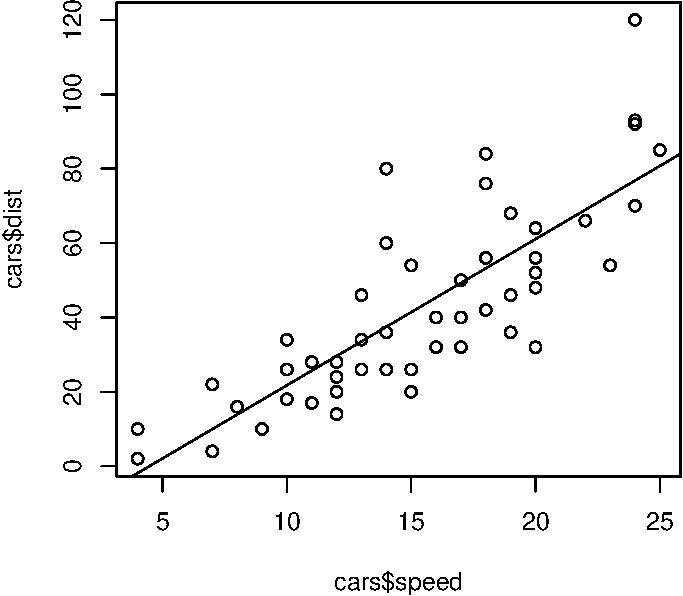
\includegraphics{visualisering_22_files/figure-latex/unnamed-chunk-28-1.pdf}

Man bruger \texttt{lm()} og huske at det skrives som \texttt{lm(y\textasciitilde{}x,data=mydata)}, hvor i dette tilfælde er x \texttt{speed} (x-aksen i ovenstående plot) og y er \texttt{dist} (y-aksen i ovenståen plot), for \texttt{mydata} = \texttt{cars}.

\begin{Shaded}
\begin{Highlighting}[]
\NormalTok{mylm }\OtherTok{\textless{}{-}} \FunctionTok{lm}\NormalTok{(dist }\SpecialCharTok{\textasciitilde{}}\NormalTok{ speed, }\AttributeTok{data=}\NormalTok{cars)  }\CommentTok{\# build linear regression model}
\NormalTok{mylm}
\end{Highlighting}
\end{Shaded}

\begin{verbatim}
## 
## Call:
## lm(formula = dist ~ speed, data = cars)
## 
## Coefficients:
## (Intercept)        speed  
##     -17.579        3.932
\end{verbatim}

\hypertarget{problemstillinger}{%
\section{Problemstillinger}\label{problemstillinger}}

\begin{enumerate}
\def\labelenumi{\arabic{enumi})}
\item
  Jeg har lavet en quiz i Absalon, hedder ``Quiz - Basics'' - som I kan starte med.
\item
  Åben en ny fil i Rstudio, ved at trykke på ``File'' \textgreater{} ``New File'' \textgreater{} ``R script''. Leger lidt - fk. nogle muligheder:
\end{enumerate}

\begin{Shaded}
\begin{Highlighting}[]
\DecValTok{2}\SpecialCharTok{+}\DecValTok{2}
\NormalTok{x }\OtherTok{\textless{}{-}} \DecValTok{4}
\NormalTok{x }\OtherTok{\textless{}{-}}\NormalTok{ x}\SpecialCharTok{+}\DecValTok{2}
\FunctionTok{sqrt}\NormalTok{(x)}
\FunctionTok{sqrt}\NormalTok{(x)}\SpecialCharTok{\^{}}\DecValTok{2}
\FunctionTok{rnorm}\NormalTok{(}\DecValTok{10}\NormalTok{,}\DecValTok{2}\NormalTok{,}\DecValTok{2}\NormalTok{)}
\FunctionTok{log10}\NormalTok{(}\DecValTok{100}\NormalTok{)}
\end{Highlighting}
\end{Shaded}

Huske at den nemmeste måde at kører kode er ved at trykke CMD+ENTER (Mac) eller WIN-KEY+ENTER (Windows).

\begin{enumerate}
\def\labelenumi{\arabic{enumi})}
\setcounter{enumi}{2}
\tightlist
\item
  Åbne op og kigge på nogle af de indbygget datasæt som vi bruger i kurset. Prøve \texttt{head()}, \texttt{summary()} osv. Prøve også fk. \texttt{?cars} for at se en beskrivelse.
\end{enumerate}

\begin{Shaded}
\begin{Highlighting}[]
\FunctionTok{data}\NormalTok{(iris)}
\FunctionTok{data}\NormalTok{(cars)}
\FunctionTok{data}\NormalTok{(sleep)}
\FunctionTok{data}\NormalTok{(PlantGrowth)}
\FunctionTok{head}\NormalTok{(chickwts)}
\CommentTok{\#se her for andre:}
\FunctionTok{library}\NormalTok{(}\AttributeTok{help =} \StringTok{"datasets"}\NormalTok{)}
\end{Highlighting}
\end{Shaded}

\begin{enumerate}
\def\labelenumi{\arabic{enumi})}
\setcounter{enumi}{3}
\tightlist
\item
  Lave en \texttt{data.frame} (dataramme) med tre kolonner som hedder ``navn'', ``alder'' og ``farve''. Sørge for, at den har 8 rækker.
\end{enumerate}

\begin{Shaded}
\begin{Highlighting}[]
\NormalTok{mydf }\OtherTok{\textless{}{-}} \FunctionTok{data.frame}\NormalTok{(}\StringTok{"navn"}\OtherTok{=}\NormalTok{ ...) }\CommentTok{\#not run, slette "..." og skrive data}
\FunctionTok{dim}\NormalTok{(mydf) }\CommentTok{\# otte række og tre kolonner}
\NormalTok{mydf}
\end{Highlighting}
\end{Shaded}

\begin{enumerate}
\def\labelenumi{\arabic{enumi})}
\setcounter{enumi}{4}
\tightlist
\item
  Lads os lave plotter i `baseR'. Vi kommer til at omdefinere hvordan vi laver plotter, når vi arbejder med \texttt{ggplot2}, men det er nyttigt at have et kendskab til baseR plotter. Jeg giver nogle muligheder for datasættet, der hedder ``iris'' - afprøve dem for nogle af de andre ovenstående indbygget datasæt, som I kiggede på.
\end{enumerate}

\begin{Shaded}
\begin{Highlighting}[]
\FunctionTok{plot}\NormalTok{(iris}\SpecialCharTok{$}\NormalTok{Sepal.Length,iris}\SpecialCharTok{$}\NormalTok{Sepal.Width)}
\FunctionTok{hist}\NormalTok{(iris}\SpecialCharTok{$}\NormalTok{Sepal.Width)}
\FunctionTok{boxplot}\NormalTok{(iris}\SpecialCharTok{$}\NormalTok{Sepal.Length}\SpecialCharTok{\textasciitilde{}}\NormalTok{iris}\SpecialCharTok{$}\NormalTok{Species)}
\end{Highlighting}
\end{Shaded}

Man kan også gøre plotterne lidt pænere ved at give dem en titel/aksen-navne osv. Prøve \texttt{?plot} for at se nogle muligheder, og tilføje \texttt{ylab}, \texttt{xlab}, \texttt{main} (titel) i én af plotterne. Lege også med \texttt{col} (farver).

\begin{enumerate}
\def\labelenumi{\arabic{enumi})}
\setcounter{enumi}{5}
\item
  Øve med at åbne en fil, der sidder i Absalon og hedder ``reactions.txt''. Kopiere filen ind i egen working directory (fk. Downloads or Documents - huske man kan sætte en working directory \texttt{setwd("\textasciitilde{}/Documents/")}) og bruge \texttt{read.table()} (giv objektet et navn, e.g.~\texttt{data}). Huske at tjekke, om filen har en `header' og bruge således \texttt{header=T} hvis nødvendigt.
\item
  Kolonner navne ``subject'' og ``condition'' indlæses som data type `int' (heltal) men skulle hellere være `factorer' (fordi de er kvalitatitiv). Gøre dem til facktorer, fk.
\end{enumerate}

\begin{Shaded}
\begin{Highlighting}[]
\NormalTok{data}\SpecialCharTok{$}\NormalTok{subject }\OtherTok{\textless{}{-}} \FunctionTok{as.factor}\NormalTok{(data}\SpecialCharTok{$}\NormalTok{subject) }\CommentTok{\#gøre subject til en faktor}
\DocumentationTok{\#\# gøre den samme her for condition:}
\NormalTok{data}\SpecialCharTok{$}\NormalTok{...}
\end{Highlighting}
\end{Shaded}

\begin{enumerate}
\def\labelenumi{\arabic{enumi})}
\setcounter{enumi}{7}
\item
  Bruge \texttt{mean} til at beregne den gennemsnitlige reaktion tid (RT) for hver af de to konditioner. Nu prøve at anvende \texttt{tapply} til at gøre den samme.
\item
  Bemærke at vores data er `paired' - det er den samme sæt ``subject''s for hver af de to ``conditions''s (altså ``subject'' = 1 har en værdi for både ``condition'' = 1 og ``condition'' = 2).
\end{enumerate}

Lave en scatter-plot af reaktioner tider mellem de to ``condition''s.

\begin{enumerate}
\def\labelenumi{\arabic{enumi})}
\setcounter{enumi}{9}
\tightlist
\item
  Lave en paired-t-test \texttt{t.test(x,y,paired=T)}. Hvad er p-værdien? Hvad er nulhypotesen og alternativ hypotesen? Er der en forskel mellem de to konditioner?
\end{enumerate}

\emph{OBS: ``reactions.txt'' er emnet af video 2 i det næste kapitel om R Markdown.}

\hypertarget{introduktion}{%
\chapter{Introduktion til R Markdown}\label{introduktion}}

\hypertarget{hvad-er-r-markdown}{%
\section{Hvad er R Markdown?}\label{hvad-er-r-markdown}}

R Markdown er ligesom R, gratis og `open source' og kan bruges som en bekvemt måde at arbejde med R til projektor på. Man kan nemlig anvende R Markdown til følgende:

\begin{itemize}
\tightlist
\item
  Skrive, gemme og køre R kode
\item
  Få direkte adgang til datasæt
\item
  Lave rapporter som kan dels med andre
\item
  En nem tilgang til at forstå andres kode, fk. gennem eksemplerne og opgaverne fra dette kursus
\end{itemize}

Vi kommer til at bruge R Markdown hele vejen igennem kurset. Man kan installere R Markdown indenfor R ved brugen af den følgende kommando:

Her er en `quick tour' som kan være nyttig (valgfri)
\url{https://rmarkdown.rstudio.com/authoring_quick_tour.html}

\hypertarget{video-demonstrationer}{%
\section{Video demonstrationer}\label{video-demonstrationer}}

Jeg har lavet to korte videoer som kan ses her.

Video 1:

\begin{itemize}
\tightlist
\item
  Jeg viser hvordan man laver et nyt dokument i R Markdown
\item
  Jeg viser hvordan man skriver tekst ind i dokumentet
\item
  Jeg viser hvordan man bruger ``knit'' til at lave en HTML-rapport
\item
  Jeg viser hvordan man oprette og køre kode chunks
\end{itemize}

Link her hvis det ikke virker nedenunder: \url{https://vimeo.com/541035944}

Video 2:

\begin{itemize}
\tightlist
\item
  Jeg viser en kort analyse med et datasæt
\item
  Jeg indlæser de data og laver en forløbig undersøgelse
\item
  Jeg laver en paired t-test og skriver konklusioner
\item
  Jeg tjekker antagelserne omkring den normal fordeling
\end{itemize}

Link her hvis det ikke virker nedenunder: \url{https://vimeo.com/541232690}

\hypertarget{lave-et-nyt-dokument-i-r-markdown}{%
\section{Lave et nyt dokument i R Markdown}\label{lave-et-nyt-dokument-i-r-markdown}}

\begin{Shaded}
\begin{Highlighting}[]
\FunctionTok{install.packages}\NormalTok{(}\StringTok{"rmarkdown"}\NormalTok{)}
\end{Highlighting}
\end{Shaded}

Huske at indlæse pakken i RStudio:

\begin{Shaded}
\begin{Highlighting}[]
\FunctionTok{library}\NormalTok{(rmarkdown)}
\end{Highlighting}
\end{Shaded}

Man åbne et nyt rmarkdown dokument ved at trykke ``New'' \textgreater{} ``New File'' \textgreater{} ``New R Markdown\ldots{}''. Man kan også trykke på den ``+'' knap øverst til venstre i hjørnet.

\begin{figure}
\centering
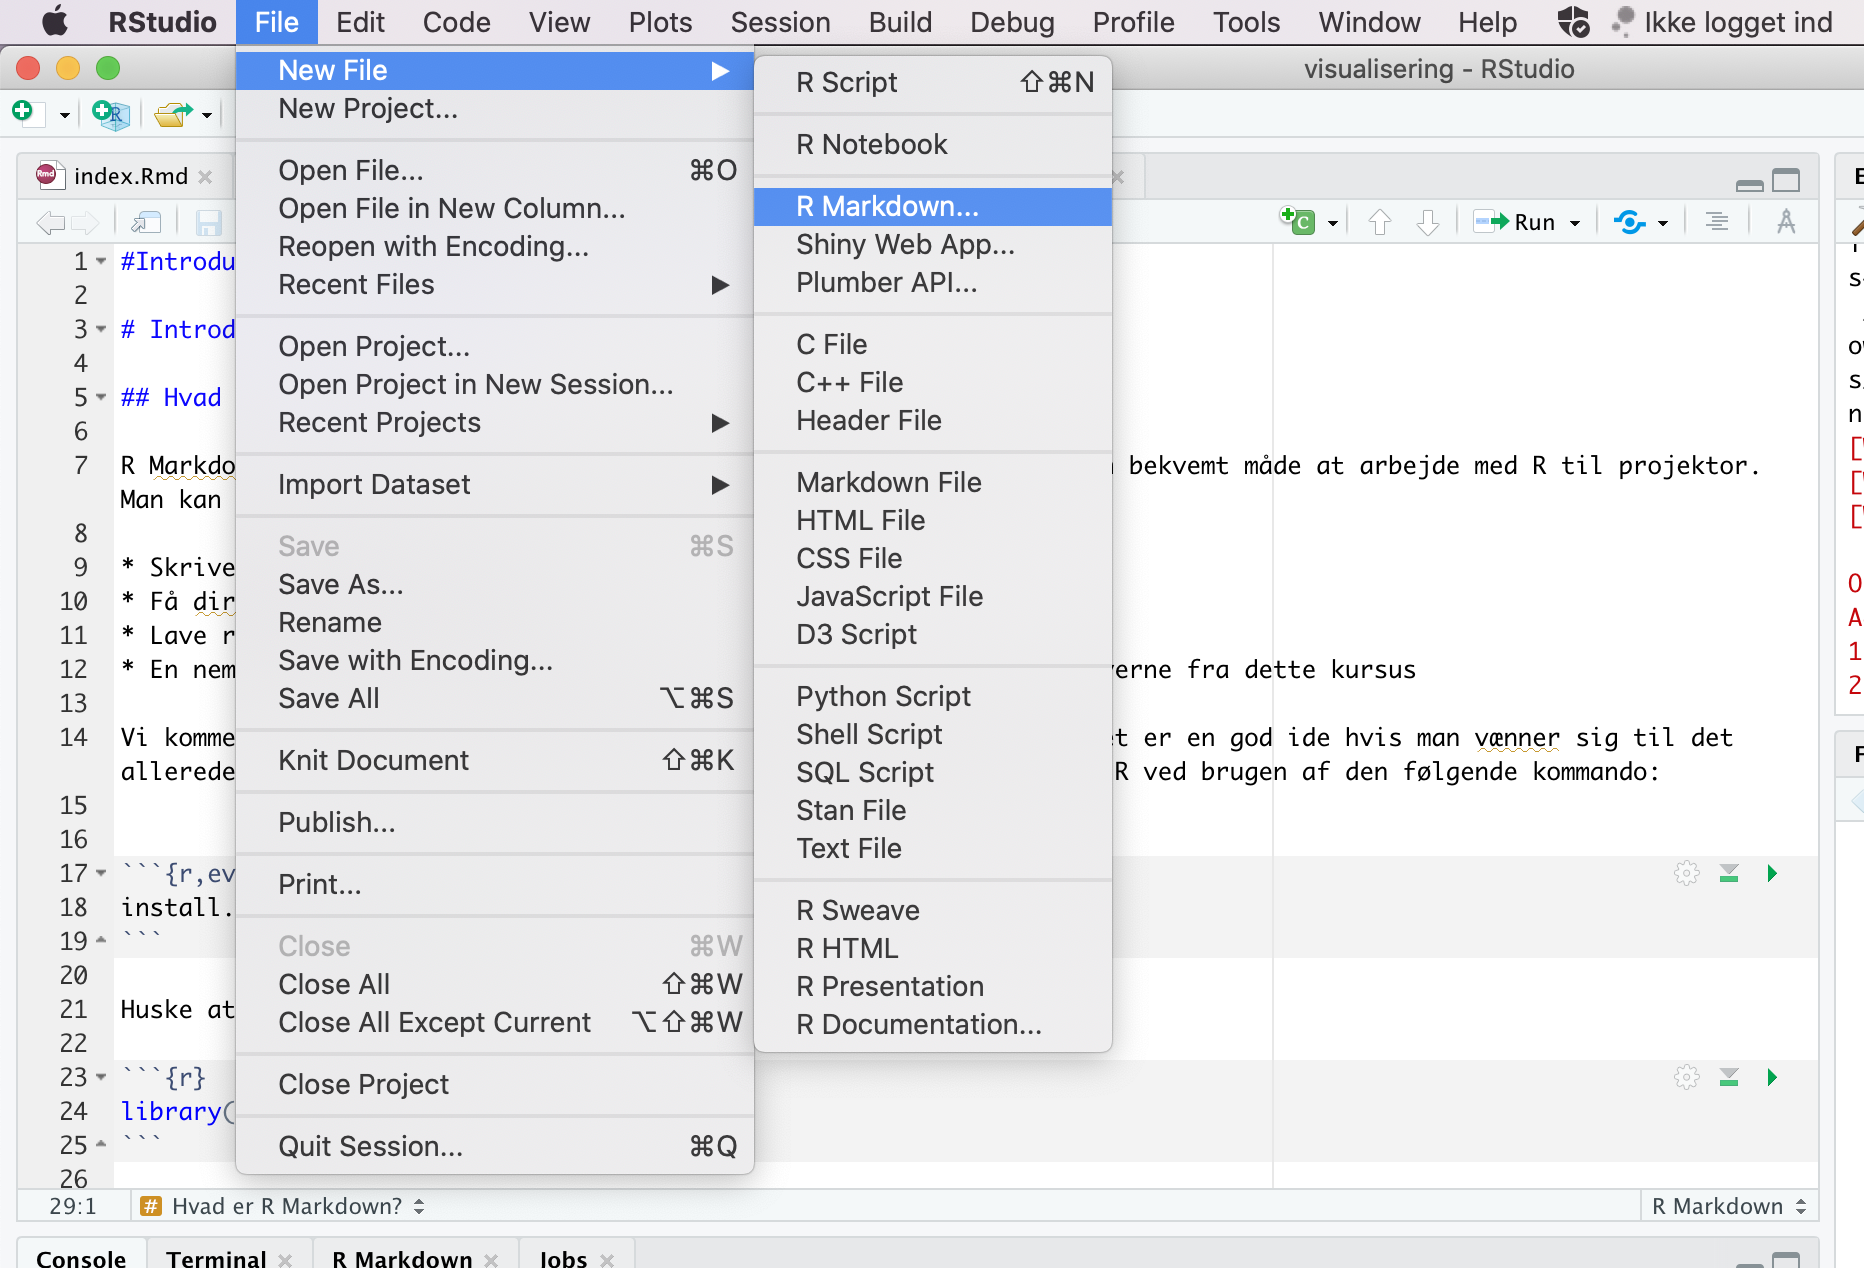
\includegraphics{plots/open_new_rmarkdown.png}
\caption{Hvordan man åbne et nyt R Markdown dokument}
\end{figure}

I de fleste tilfælde arbejder vi med HTLM dokumenter, men man har også andre muligheder (PDF/Word/Shiny osv\ldots).

\begin{figure}
\centering
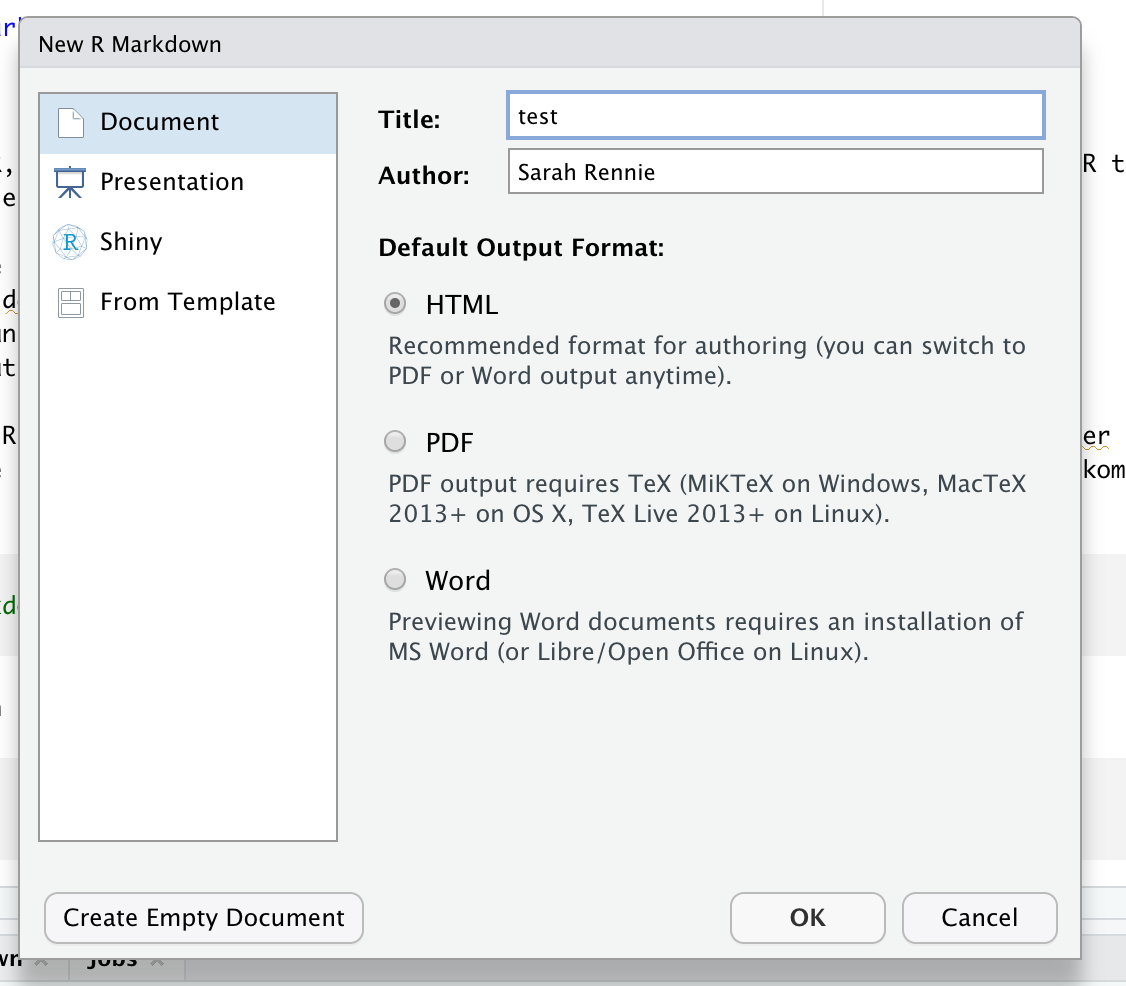
\includegraphics{plots/create_new_rmarkdown.png}
\caption{Hvordan man åbne et nyt R Markdown dokument}
\end{figure}

\hypertarget{yaml}{%
\subsection{YAML}\label{yaml}}

Den første sektion hedder `YAML'. (Dette står for `YAML Ain't Markup Language').

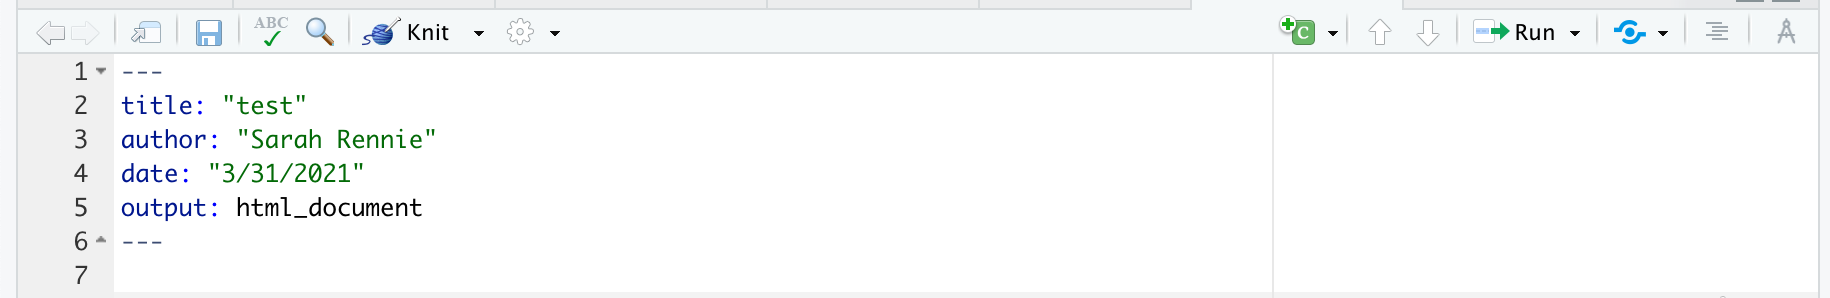
\includegraphics{plots/YAML.png}
Det indeholder oplysninger om dokumentet, og her kan man specificere forskellige muligheder - fk. titel, forfatter, output-type (fks. HTML eller PDF), datoen, osv.

I de fleste tilfælde, kan vi bare nøjes med at bruge standard indstillinger, men hvis man gerne vil lære mere om de forskellige muligheder med YAML, kan man læse her:

\url{https://bookdown.org/yihui/rmarkdown/html-document.html}

eller se en liste muligheder her på den her cheatsheet:

\url{https://www.rstudio.com/wp-content/uploads/2016/03/rmarkdown-cheatsheet-2.0.pdf}

\hypertarget{globale-options}{%
\subsection{Globale options}\label{globale-options}}

Bemærke, at der også er nogle tekst som ser ud som følgende:

\begin{figure}
\centering
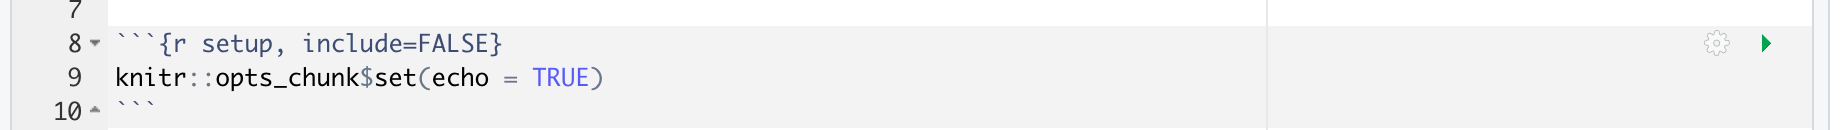
\includegraphics{plots/global_options.png}
\caption{Hvordan man åbner et nyt R Markdown dokument}
\end{figure}

Med funktionen \texttt{opts\_chunk\$set()} kan man specificere de globale indstillinger, man gerne vil have, som styrer hvordan det færdige dokument ser ud. I dette tilfælde, er de fleste parametre angivet som `default' (da de ikke er nævnt eksplicit), og \texttt{echo} er den eneste der har noget andet angivet. Hvis \texttt{echo} er \texttt{TRUE}, så betyder det, at når man kører sine kode og kompilerer dokumentet, så kan man også se den kode, der blev kørte, ligesom dens output, som en del af den færdige HTML, der fremvises.

\hypertarget{skrive-baserende-tekst}{%
\section{Skrive baserende tekst}\label{skrive-baserende-tekst}}

Her er nogle nyttige måder, man kan skrive tekste på, i opgaverne eller rapporter.

\begin{Shaded}
\begin{Highlighting}[]
\SpecialCharTok{*}\NormalTok{italic}\SpecialCharTok{*}   \ErrorTok{**}\NormalTok{bold}\SpecialCharTok{**}

\NormalTok{\_italic\_   \_\_bold\_\_}
\end{Highlighting}
\end{Shaded}

\emph{italic} \textbf{bold}

\emph{italic} \textbf{bold}

\hypertarget{headers}{%
\subsection{Headers}\label{headers}}

Man kan også lave sektioner:

\begin{Shaded}
\begin{Highlighting}[]
\CommentTok{\# Header 1}

\DocumentationTok{\#\# Header 2}

\DocumentationTok{\#\#\# Header 3}
\end{Highlighting}
\end{Shaded}

\begin{figure}
\centering
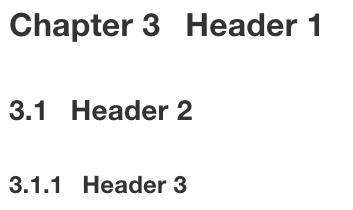
\includegraphics{header_eksempel.png}
\caption{Caption for the picture.}
\end{figure}

\hypertarget{liste}{%
\subsection{liste}\label{liste}}

\begin{Shaded}
\begin{Highlighting}[]
\SpecialCharTok{*}\NormalTok{ Item }\DecValTok{1}
\SpecialCharTok{*}\NormalTok{ Item }\DecValTok{2}
    \SpecialCharTok{+}\NormalTok{ Item 2a}
    \SpecialCharTok{+}\NormalTok{ Item 2b}
\end{Highlighting}
\end{Shaded}

\begin{itemize}
\tightlist
\item
  Item 1
\item
  Item 2

  \begin{itemize}
  \tightlist
  \item
    Item 2a
  \item
    Item 2b
  \end{itemize}
\end{itemize}

\hypertarget{kode-indenfor-teksten-inline-chunks}{%
\section{Kode indenfor teksten (`Inline chunks')}\label{kode-indenfor-teksten-inline-chunks}}

De fleste vores kode skrives indenfor såkaldte `chunks' som vi kommer til nedenfor. Men nogle gange kan det være nyttigt at skrive kode direkte indenfor teksten. Dette gøres ved at skrive

\begin{Shaded}
\begin{Highlighting}[]
\NormalTok{Her er nogle }\StringTok{\textasciigrave{}}\AttributeTok{kode}\StringTok{\textasciigrave{}}
\end{Highlighting}
\end{Shaded}

som ser sådan ud indenfor teksten:

Her er nogle \texttt{kode}

I dette tilfælde, bliver koden ikke kørte. Hvis man vil køre koden indenfor teksten, kan man skrive (for eksempel):

\begin{Shaded}
\begin{Highlighting}[]
\NormalTok{De gennemsnitlige antal af observationer er }\StringTok{\textasciigrave{}}\AttributeTok{r mean(c(5,7,4,6,3,3))}\StringTok{\textasciigrave{}}
\end{Highlighting}
\end{Shaded}

som ser sådan ud indenfor teksten:

De gennemsnitlige antal af observationer er 4.6666667

Og hvis man dropper de `r', så bliver kodet ikke kørte:

\begin{Shaded}
\begin{Highlighting}[]
\NormalTok{De gennemsnitlige antal af observationer er }\StringTok{\textasciigrave{}}\AttributeTok{mean(c(5,7,4,6,3,3))}\StringTok{\textasciigrave{}}
\end{Highlighting}
\end{Shaded}

giver:

De gennemsnitlige antal af observationer er \texttt{mean(c(5,7,4,6,3,3))}

\hypertarget{kode-chunks}{%
\section{Kode chunks}\label{kode-chunks}}

Man kan oprette en ny chunk, enten ved at trykke på de \emph{Insert a new code chunk} knap ovenpå, eller ved at trykke \emph{Cmd+Option+I} på tastaturet (hvis man bruger MAC) eller \emph{Ctrl+Alt+I} (hvis man bruger Windows).

Tryk på den grønne pile, der hedder \emph{Run current chunk} for at køre hele den chunk. Resultatet kan ses lige nedenunder. Man kan også trykke på den grønne pile som ligger øverst til højre i den kode chunk.

Det er ofte hurtigere at bruge \emph{Run current chunk} i stedet for at \emph{Knit} (se nedenfor) hver gang man vil køre kode, fordi her kører man kun den enkele chunk, man er interesset i, i stedet for det hele dokument (som er tilfældet med \emph{Knit}).

\hypertarget{chunk-options}{%
\subsection{Chunk options}\label{chunk-options}}

For eksempel, en chunk med en `option' nævnt ser sådan ud (fjerne \# symbol)

\begin{Shaded}
\begin{Highlighting}[]
\CommentTok{\#\textasciigrave{}\textasciigrave{}\textasciigrave{}\{r,eval=FALSE\}}
\CommentTok{\#}
\CommentTok{\#\textasciigrave{}\textasciigrave{}\textasciigrave{}}
\end{Highlighting}
\end{Shaded}

Her er nogle muligheder (sektionen ``Embed code with knitr syntax''):

\url{https://www.rstudio.com/wp-content/uploads/2016/03/rmarkdown-cheatsheet-2.0.pdf}

Her er seks populær muligheder som jeg har kopiret fra nettet:

\begin{itemize}
\tightlist
\item
  \texttt{include\ =\ FALSE}

  \begin{itemize}
  \tightlist
  \item
    prevents code and results from appearing in the finished file. R Markdown still runs the code in the chunk, and the results can be used by other chunks.
  \end{itemize}
\item
  \texttt{echo\ =\ FALSE}

  \begin{itemize}
  \tightlist
  \item
    prevents code, but not the results from appearing in the finished file. This is a useful way to embed figures.
  \end{itemize}
\item
  \texttt{message\ =\ FALSE}

  \begin{itemize}
  \tightlist
  \item
    prevents messages that are generated by code from appearing in the finished file.
  \end{itemize}
\item
  \texttt{warning\ =\ FALSE}

  \begin{itemize}
  \tightlist
  \item
    prevents warnings that are generated by code from appearing in the finished.
  \end{itemize}
\item
  \texttt{fig.cap\ =\ "..."}

  \begin{itemize}
  \tightlist
  \item
    adds a caption to graphical results.
  \end{itemize}
\item
  \texttt{eval\ =\ FALSE}

  \begin{itemize}
  \tightlist
  \item
    does not evaluate the code
  \end{itemize}
\end{itemize}

\hypertarget{knit-kode}{%
\section{Knit kode}\label{knit-kode}}

Man bruger \emph{Knit} for at gengive filen i HTML form. Når man trykke på \emph{Knit}, alle kode i filen bliver kørte og en HTML fremviser.

Man kan også bruge \emph{Preview}, som kører ikke kode chunks, men bruger koden som blev kørt før.

\hypertarget{matematik}{%
\section{Matematik}\label{matematik}}

For example, the inline code \texttt{\$\textbackslash{}int\_0\^{}5\ x\^{}2\ dx\$} will typeset as \(\int_0^5 x^2 dx\):

\hypertarget{problemstillinger-1}{%
\section{Problemstillinger}\label{problemstillinger-1}}

\begin{enumerate}
\def\labelenumi{\arabic{enumi})}
\item
  Jeg har lavet en kort \textbf{quiz} i Absalon, som hedder ``Quiz - R Markdown''.
\item
  Lave et nyt R Markdown dokument i R Studio. Prøve at lave en list og nogle overskrifter af forskellige størrelser.
\item
  Tryk på \texttt{Knit} og tjekke at et html-dokument fremvises som forventet.
\item
  Tilføj en ny R chunk, med noget kode. e.g.
\end{enumerate}

\begin{Shaded}
\begin{Highlighting}[]
\NormalTok{x }\OtherTok{\textless{}{-}} \FunctionTok{rnorm}\NormalTok{(}\DecValTok{20}\NormalTok{,}\DecValTok{1}\NormalTok{,}\DecValTok{2}\NormalTok{) }\CommentTok{\#make a sample of normally distributed data}
\FunctionTok{plot}\NormalTok{(x)}
\end{Highlighting}
\end{Shaded}

Øve med at trykke enten på den grønne pile, eller på knit.

\begin{enumerate}
\def\labelenumi{\arabic{enumi})}
\setcounter{enumi}{4}
\tightlist
\item
  Bruge \texttt{\$\ \$} til at skrive formulen til `mean' ind i teksten, \(\bar{x}\). Hint: \texttt{\$\textbackslash{}sum\_\{i=1\}\^{}\{n\}\$} and \texttt{\$\{x\_\{i\}\}\$}.
\end{enumerate}

\hypertarget{opgaven}{%
\section{Opgaven}\label{opgaven}}

Huske at sende mig eventuelle spørgsmål, som jeg kan svare på i Zoom rummet (sende gerne via mail eller chat).

Ind på Absalon har jeg lagt en R Markdown fil som hedder ``R Markdown opgave'', som I kan bruge til at starte med at arbejde lidt med R Markdown baserede opgaver. Det kombinerer koncepter fra de forudgående kapitel om de grundlæggende ting i R og statistik.

\hypertarget{slut-for-ugen}{%
\section{Slut for ugen}\label{slut-for-ugen}}

Næste gang begynder vi at arbejde vi med \texttt{ggplot2}.

\hypertarget{ekstra-links}{%
\section{Ekstra links}\label{ekstra-links}}

\url{https://www.rstudio.com/wp-content/uploads/2015/03/rmarkdown-reference.pdf?_ga=2.49295910.1034302809.1602760608-739985330.1601281773}

  \bibliography{book.bib,packages.bib}

\end{document}
